% Created 2026-05-26 Tue 00:03
\documentclass{article}
\usepackage[utf8]{inputenc}
\usepackage[T1]{fontenc}
\usepackage{graphicx}
\usepackage{longtable}
\usepackage{wrapfig}
\usepackage{rotating}
\usepackage[normalem]{ulem}
\usepackage{amsmath}
\usepackage{amssymb}
\usepackage{capt-of}
\usepackage{hyperref}

\usepackage{fancyhdr}
\usepackage[top=25mm, left=25mm, right=25mm]{geometry}
\usepackage{longtable}
\fancyhead[R]{}
\setlength\headheight{43.0pt}
\usepackage{tabularx}
\usepackage{longtable}
\usepackage[backend=biber, style=ieee]{biblatex}
\addbibresource{/home/josejacome_epn/bibliography/bibliography.bib}
\author{-Leonardo Shande Rodriguez Chaci}
\date{[26/05/2026]}
\title{Taller - Conceptos Básicos de Hardware y Ensamblaje de Computadores\\\medskip
\large ICCD332 Arquitectura de Computadores }
\hypersetup{
 pdfauthor={-Leonardo Shande Rodriguez Chaci},
 pdftitle={Taller - Conceptos Básicos de Hardware y Ensamblaje de Computadores},
 pdfkeywords={},
 pdfsubject={},
 pdfcreator={Emacs 29.3 (Org mode 9.6.15)}, 
 pdflang={Spanish}}
\begin{document}

\maketitle
\begin{itemize}
\item 
\end{itemize}
\fancyhead[C]{
\includegraphics[scale=0.05]{../images/logoEPN.jpg}\\
ESCUELA POLITECNICA NACIONAL\\FACULTAD DE INGENIERIA DE SISTEMAS\\
ARQUITECTURA DE COMPUTADORES}
\thispagestyle{fancy}


\section{Instrucciones generales}
\label{sec:orgc4f6d54}

Este taller se realiza en \textbf{grupos}. Cada integrante debe completar
individualmente el curso Cisco Networking Academy:
\textbf{Conceptos Básicos de Hardware de Computadora} y obtener su
certificado de completitud. 

\textbf{Entregables del grupo:}
\begin{itemize}
\item Resolución de éste archivo fuente \texttt{.org}
\item El PDF exportado desde Emacs \texttt{M-x org-latex-export-to-pdf}
\item Los certificados individuales de cada integrante (PDF o imagen)
\end{itemize}


\textbf{Entregable Individual(Tarea):}
\begin{itemize}
\item Resolver el cuestionario individual en el aula virtual
\end{itemize}
\subsection{Recursos}
\label{sec:org9eaff18}
Cree su usuario en la plataforma de \emph{Cisco Networking Academy}. Use el
siguiente enlace:

\href{https://www.netacad.com/es/courses/computer-hardware-basics?courseLang=en-US}{Cisco Computer Hardware Basics}

Puede configurar según el idioma de su preferencia. El texto está
disponible en Español. Los vídeos disponen de subtítulos en varios
idiomas.

\section{Parte A. Integrantes y certificados}
\label{sec:org1f2b1b4}
Para insertar la captura del certificado utilice YASnippet: Escriba
\texttt{fig\_} seguido de \texttt{C-TAB}. Esto produce \texttt{\#+caption}, \texttt{\#+attr\_latex} y
\texttt{\#+label} que permiten colocar un encabezado a la imagen, controlar el
escalado de la misma y una referencia. Finalmente inserte el enlace al
archivo usando \texttt{C-c C-l} o usando \texttt{[[./carpeta-certificados/cert-int1.pdf]]}
\begin{enumerate}
\item \textbf{Integrante 1}
\begin{itemize}
\item \textbf{Nombre completo:}
Leonardo Shande Rodriguez Chaci
\item \textbf{Correo:}
leonardo.rodriguez01@epn.edu.ec
\item \textbf{Certificado adjunto:}

[[\begin{figure}[htbp]
\centering
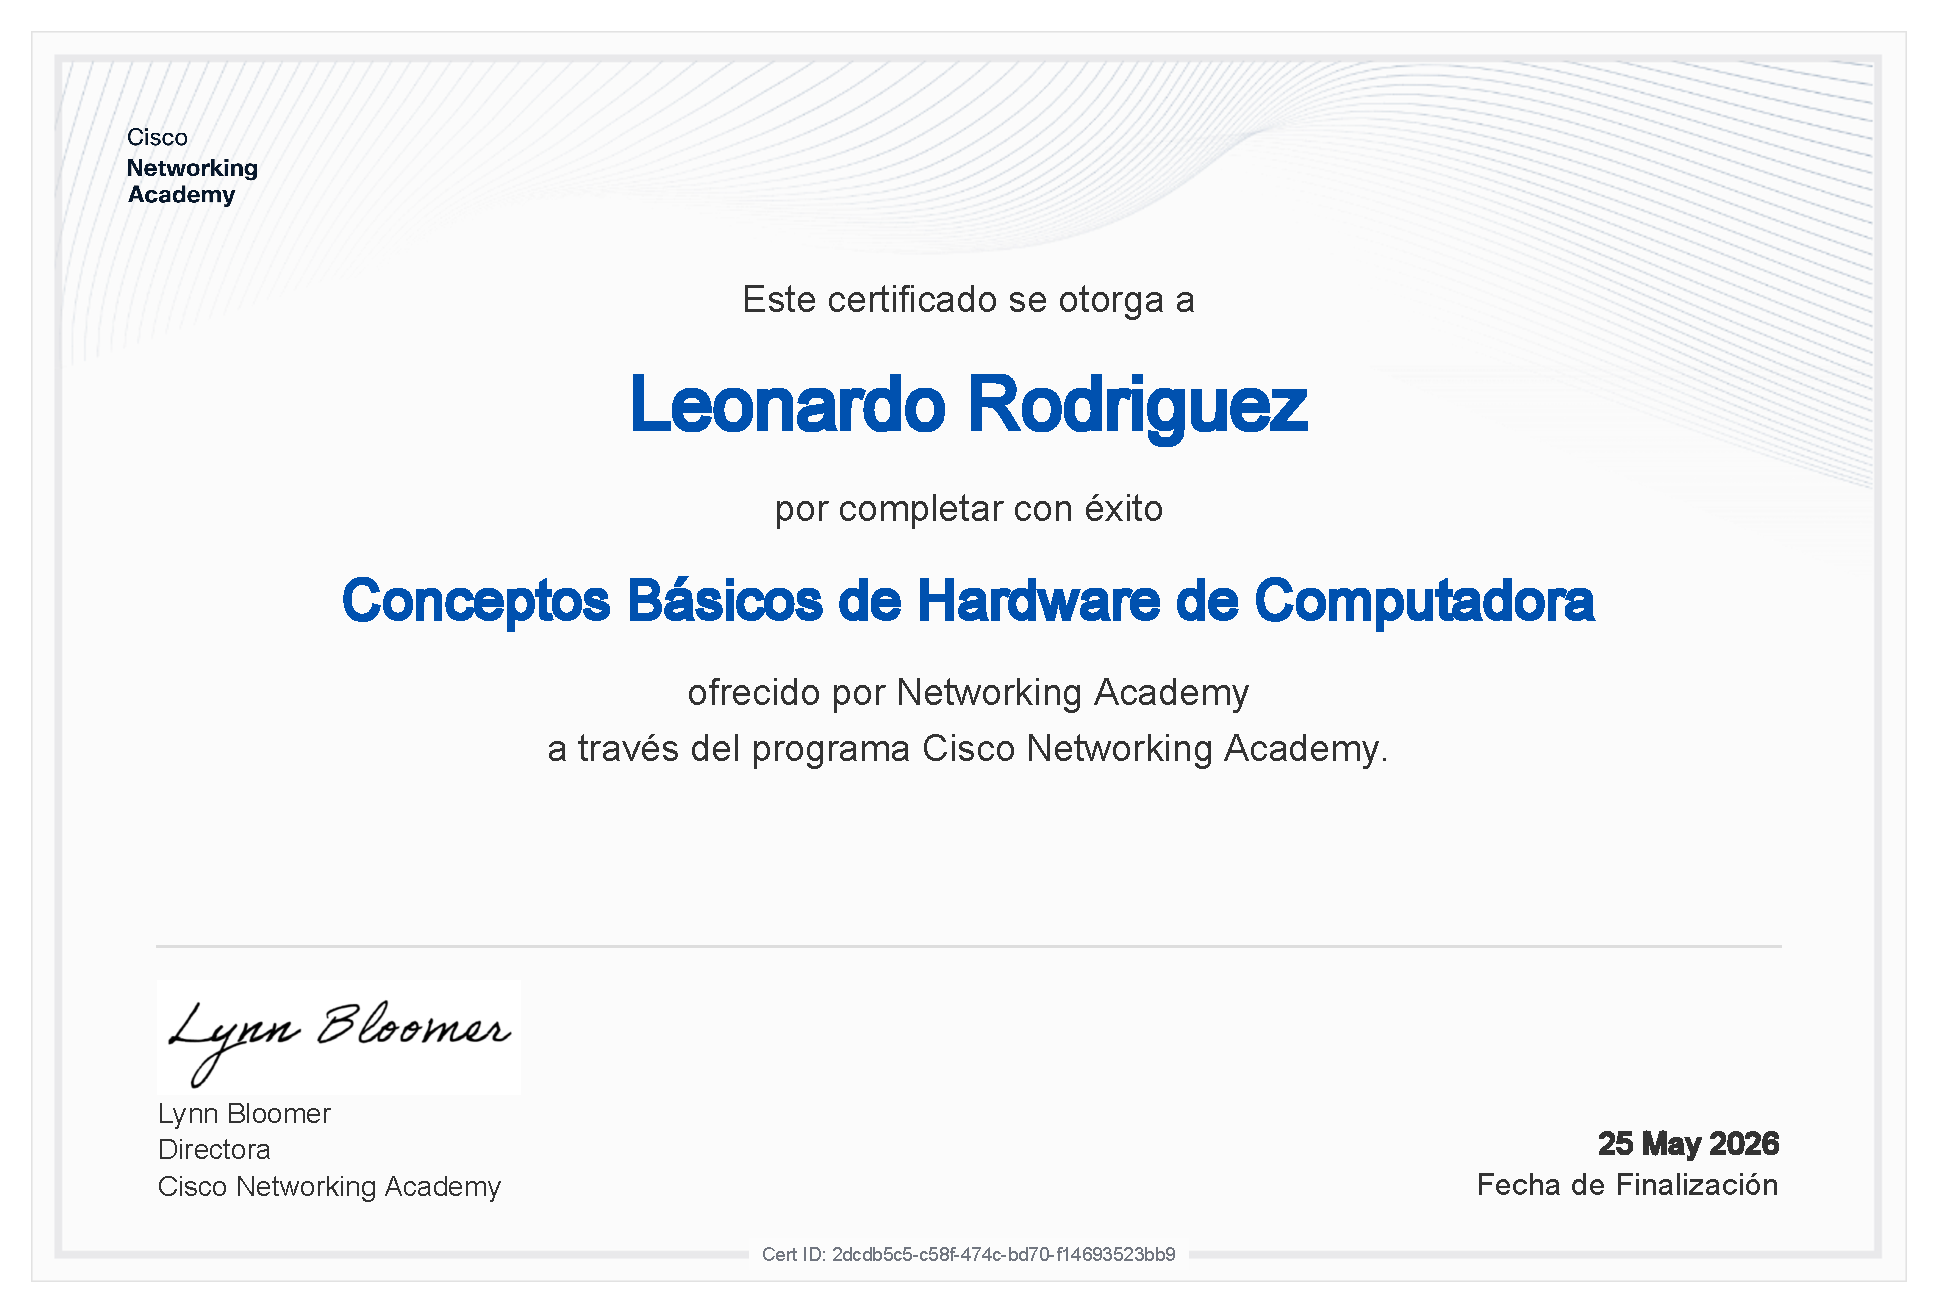
\includegraphics[width=.9\linewidth]{Fotos/Computer_Hardware_Basics_certificate_leonardo-rodriguez01-epn-edu-ec_2dcdb5c5-c58f-474c-bd70-f14693523bb9.pdf}
\caption{\label{fig:org8a3dfe5}Certificado de Leonardo Rodriguez}
\end{figure}]]
\end{itemize}

\item \textbf{Integrante 2}
\begin{itemize}
\item \textbf{Nombre completo:}
José Manuel Jácome Navarrete
\item \textbf{Correo:}
jose.jacome04@epn.edu.ec
\end{itemize}
\end{enumerate}
\subsection{\textbf{Certificado adjunto:}}
\label{sec:org63e0b03}

\vspace{-0.5cm}
[[\begin{center}
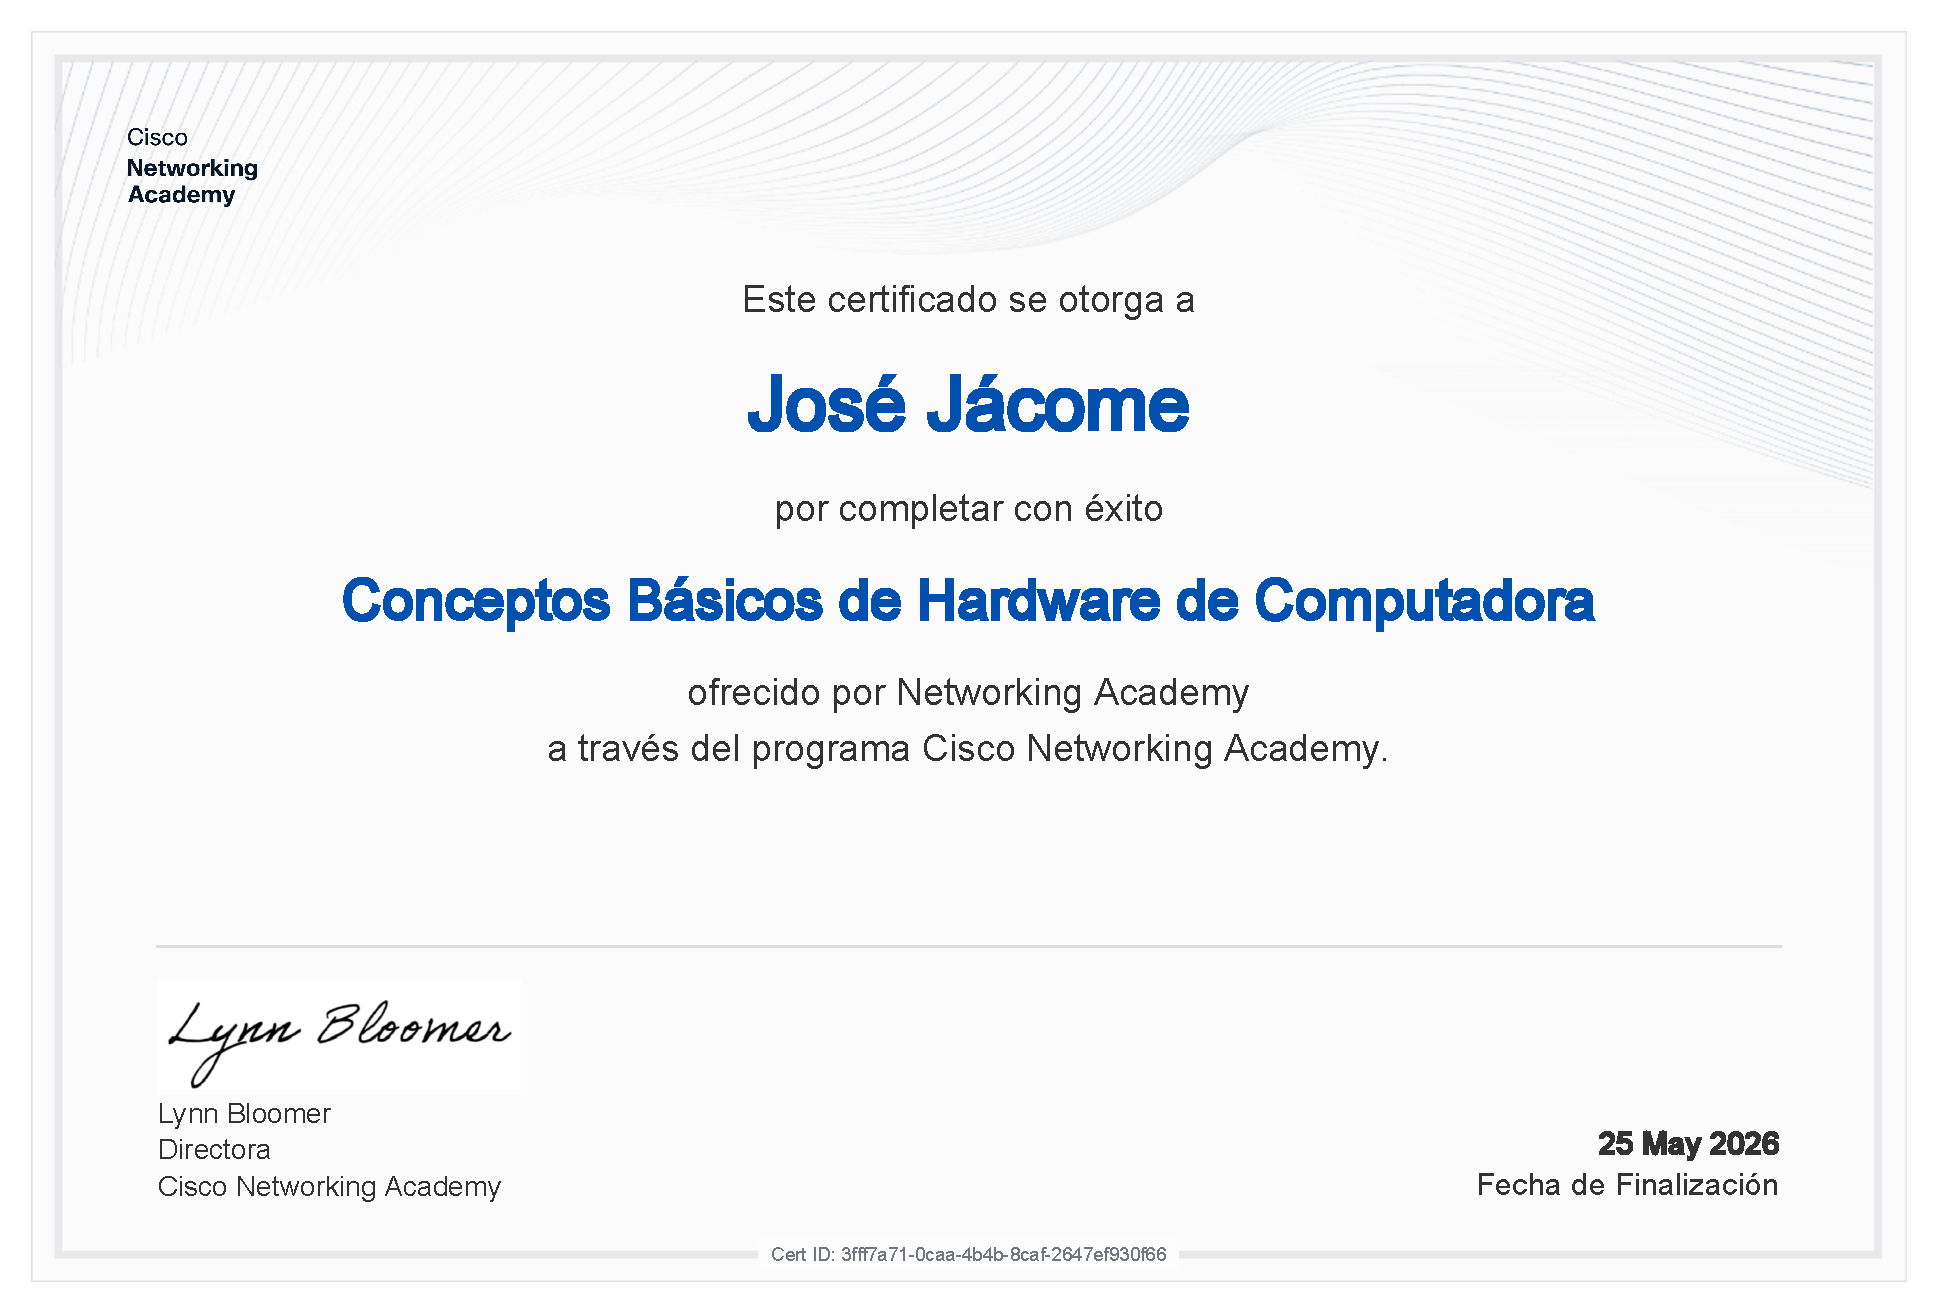
\includegraphics[width=.9\linewidth]{Fotos/Computer-Hardware-Basics-certificate-jose-3fff7a71-0caa-4b4b-8caf-2647ef930f66.pdf.pdf}
\end{center}]]

\begin{enumerate}
\item \textbf{Integrante 3}
\begin{itemize}
\item \textbf{Nombre completo:}
\item \textbf{Usuario institucional:}
\item \textbf{Correo:}
\item \textbf{Certificado adjunto:} (sí / no)
\begin{verbatim}
      Siga las instrucciones para insertar la imagen usando YASnippet
\end{verbatim}
\end{itemize}
\end{enumerate}

\section{Parte B. Cuestionario argumentado grupal}
\label{sec:org652e82c}

Para cada pregunta:

\begin{itemize}
\item Indique la alternativa escogida (letra).
\item Escriba una justificación técnica breve (3 a 6 líneas). Fundamente
su respuesta. Su insumo principal es el curso de Conceptos Básicos
de Hardware. Si usa otro material referenciar.
\item Discuta con el grupo de trabajo las opciones y la respuesta ¿Existió
consenso? ¿Cuáles fueron las principales discrepancias?
\end{itemize}

\textbf{Criterio:} correcto/incorrecto + calidad del argumento técnico.

\subsection{Pregunta 1}
\label{sec:org0712e54}
Al instalar una CPU en un socket LGA, ¿por qué es crítico alinear el
pin 1 de la CPU con el pin 1 del socket?

a. Para que el sistema arranque con mayor rapidez 

b. Para evitar daños en la CPU y el socket al insertar incorrectamente

c. Porque el pin 1 es el único que conduce electricidad 

d. Para que el disipador quede centrado automáticamente

\begin{itemize}
\item \emph{Alternativa escogida:} [b]

\item \emph{Justificación técnica:} [La alineación del pin 1 es crítica porque
los sockets LGA contienen pines extremadamente
delicados en la placa base que hacen contacto con las almohadillas
de la CPU. Una inserción incorrecta o forzada debido a una mala
orientación puede doblar o romper de forma irreversible los pines
del socket, destruyendo la conectividad eléctrica de la placa o
cortocircuitando el procesador. Los fabricantes incluyen guías
físicas y un triángulo indicador en la esquina del chip
precisamente para prevenir este daño mecánico.]

\item \emph{Debate del grupo:} [No existieron discrepancias fundamentales, ya
que todos los integrantes coincidimos en que un error de orientación
en un socket LGA produce daños físicos directos en el hardware,
descartando las opciones de software o velocidad.]
\end{itemize}

\subsection{Pregunta 2}
\label{sec:org26b32e9}
Al montar la placa madre en el gabinete, ¿cuál es la función de los separadores (standoffs)?

a. Sostener el peso de las tarjetas de expansión

b. Evitar cortocircuitos entre la placa madre y el metal del gabinete

c. Mejorar la ventilación de la placa madre

d. Facilitar la alineación del panel de E/S trasero

\begin{itemize}
\item \emph{Alternativa escogida:} [b]

\item \emph{Justificación técnica:} [Los separadores o standoffs son pequeñas
piezas metálicas o de plástico que se atornillan al chasis del
gabinete antes de colocar la placa madre. Su función principal es
aislar eléctricamente la parte posterior de la PCB de la
superficie metálica conductora del gabinete. Si la placa madre
tocara directamente el chasis, se generarían múltiples
cortocircuitos al encender el equipo, lo que podría quemar
componentes críticos como el chipset, las fases de poder o el
procesador.]

\item \emph{Debate del grupo:} [Existió un consenso absoluto y unánime en el
grupo. No hubo discrepancias, puesto que recordamos que el metal del
gabinete es un conductor eléctrico y que la separación física es la
única medida estándar de seguridad para prevenir fallas
catastróficas por corto circuito durante el ensamblaje.]
\end{itemize}

\subsection{Pregunta 3}
\label{sec:orgfa9761c}
Según el manual de ensamblaje de Cisco, ¿cuándo NO es necesario aplicar pasta térmica al instalar el disipador sobre la CPU?

a. Cuando la CPU es de alto rendimiento

b. Cuando el disipador ya incluye pasta térmica preaplicada

c. Cuando la CPU tiene más de un año de uso

d. Cuando el gabinete tiene buena ventilación

\begin{itemize}
\item \emph{Alternativa escogida:} [b]

\item \emph{Justificación técnica:} [No es necesario aplicar pasta térmica
manual si el disipador de fábrica ya cuenta con una
almohadilla térmica o pasta preaplicada en su base de cobre o
aluminio. Colocar pasta adicional sobre una superficie que ya la
incluye genera una capa excesivamente gruesa que actúa como aislante
térmico en lugar de conductor, empeorando drásticamente la
transferencia de calor hacia las aletas del disipador. El manual de
Cisco especifica que solo se debe aplicar pasta térmica manualmente
tras limpiar por completo cualquier residuo anterior utilizando
alcohol isopropílico.]

\item \emph{Debate del grupo:} [Tuvimos un consenso pleno en el grupo tras
recordar las guías de ensamblaje estándar. Coincidimos en que la
duplicación de compuestos térmicos satura el área de contacto y
eleva peligrosamente las temperaturas de la CPU, descartando por
unanimidad las demás opciones relacionadas con el tiempo de uso o la
ventilación del gabinete.]
\end{itemize}

\subsection{Pregunta 4}
\label{sec:org95a382b}
¿Por qué se recomienda usar pulsera antiestática y alfombrilla antiestática al manipular componentes internos?

a. Para proteger al técnico de descargas de 220 V

b. Para evitar que la electricidad estática dañe los componentes

c. Para cumplir una norma estética del laboratorio

d. Para que los tornillos no se magneticen

\begin{itemize}
\item \emph{Alternativa escogida:} [b]

\item \emph{Justificación técnica:} [El cuerpo humano puede acumular miles de
voltios de electricidad estática a través de la fricción diaria. Al
tocar componentes semiconductores extremadamente sensibles, esa
carga puede liberarse repentinamente en forma de una descarga
electrostática. Esto puede destruir instantáneamente los
microcircuitos internos o causar daños latentes que degraden el
hardware con el tiempo. La pulsera y la alfombrilla antiestática
crean una vía segura y continua a tierra, disipando la carga de
forma controlada antes de que pueda saltar al hardware.]

\item \emph{Debate del grupo:} [Hubo un consenso rápido y sin discrepancias en
el grupo. Todos estuvimos de acuerdo en que la alternativa "a" es
incorrecta porque estos elementos no protegen contra voltajes altos
de la línea eléctrica, y las opciones "c" y "d" no tienen fundamento técnico
sobre la protección de circuitos.]
\end{itemize}

\subsection{Pregunta 5}
\label{sec:orgdc1aee0}
Si al iniciar la computadora por primera vez un LED del panel frontal no funciona, ¿qué indica el manual de Cisco?

a. Reemplazar el conector por uno de repuesto

b. Revisar el BIOS para habilitar el LED

c. Quitar el conector, invertirlo y volver a conectarlo

d. Desconectar y reconectar la fuente de poder

\begin{itemize}
\item \emph{Alternativa escogida:} [c]

\item \emph{Justificación técnica:} [Los diodos emisores de luz del panel
frontal funcionan con corriente continua y poseen polaridad, lo que
significa que tienen un polo positivo y uno negativo. Si el conector
del panel frontal se conecta al revés en los pines de la placa
madre, el diodo quedará polarizado en inversa y la corriente no
podrá fluir, impidiendo que el LED se encienda. El manual de Cisco
indica que ante este fallo común no se debe asumir un daño de
fábrica, sino simplemente desconectar el jumper, invertir su
orientación y volver a conectarlo para corregir
la polaridad.]

\item \emph{Debate del grupo:} [Hubo consenso total en el grupo. Al debatir las
opciones, descartamos "b" porque el BIOS no controla individualmente
los LEDs físicos del chasis, y "a" o "d" serían medidas
desproporcionadas antes de verificar algo tan básico en el
ensamblaje de hardware como la orientación de los cables de
control.]
\end{itemize}

\subsection{Pregunta 6}
\label{sec:org5f2c660}
¿Por qué una GPU puede requerir un conector de alimentación PCIe adicional de la fuente de poder?

a. Porque la ranura PCIe no transmite señal de video

b. Porque las GPUs de alto rendimiento consumen más potencia de la que la ranura puede suministrar

c. Porque el conector PCIe solo funciona con tarjetas de red

d. Por el estándar de codificación de color de los cables SATA

\begin{itemize}
\item \emph{Alternativa escogida:} [b]

\item \emph{Justificación técnica:} [La ranura PCIe x16 de la placa madre está
limitada por estándar a suministrar un máximo de 75W de potencia
eléctrica. Las tarjetas gráficas de gama media y alta dedicadas al
procesamiento complejo de gráficos o videojuegos consumen mucha más
energía de la que esa ranura puede proveer de forma segura. Para
suplir este déficit y evitar sobrecargar los circuitos de la placa,
las fuentes de poder incluyen cables de alimentación dedicados que
entregan energía directa de las líneas de +12V para garantizar la
estabilidad del sistema bajo carga.]

\item \emph{Debate del grupo:} [En el grupo existió consenso absoluto sobre la
opción "b". Al revisar los fundamentos de hardware, descartamos
inmediatamente la "a" porque el bus PCIe sí maneja el tráfico de
datos de video hacia el procesador, la "c" porque no está limitado a
tarjetas de red, y la "d" porque mezcla de forma errónea los
estándares de almacenamiento SATA con los de alimentación gráfica.]
\end{itemize}

\section{Parte C. Mantenimiento de computadores}
\label{sec:org4f7ae37}

\subsection{3.1 Insumos para mantenimiento preventivo}
\label{sec:orgee55e7a}
Liste al menos seis insumos y describa para qué sirve cada
uno. Revise el siguiente \href{https://youtu.be/3ri1BMV7XTM?si=bjYoDUUKuMWwj4Qg}{vídeo}.

\begin{center}
\begin{tabular}{ll}
Insumo & Uso principal\\[0pt]
\hline
Aire Comprimido & Remover polvo en ventiladores y puertos.\\[0pt]
Alcohol isopropílico & Limpiar componentes electrónicos.\\[0pt]
Brocha antiestática & Limpiar el polvo de partes delicadas.\\[0pt]
Pasta térmica & Mejorar la disipación de calor del procesador.\\[0pt]
Destornillador & Abrir el equipo correctamente.\\[0pt]
Paño de microfibra & Limpiar pantallas.\\[0pt]
\end{tabular}
\end{center}

\subsection{3.2 Procedimiento de limpieza — Desktop}
\label{sec:org5dbed30}
\begin{enumerate}
\item Apagar el computador, desconectarlo de la corriente y tomar en
cuenta las medidas antiestática.
\item Abrir el gabinete usando las herramientas necesarias, ver el
estado de los componentes y el polvo.
\item Limpiar ventiladores, disipadores, fuente de poder y tarjetas
con la brocha antiestática y el aire comprimido.
\item Limpiar las superficies con paño de microfibra y alcohol
isopropílico, evitando usar líquido en los componentes directamente.
\item Verificar la correcta conexión de cables y componentes, cerrar
el gabinete y verificar que todo funcione correctamente.
\end{enumerate}

\subsection{3.3 Procedimiento de limpieza — Laptop}
\label{sec:orgd6ecf42}
\begin{enumerate}
\item 

\item 

\item 

\item 

\item 
\end{enumerate}

\section{Parte D. Aprendizaje obtenido}
\label{sec:orgc7f1ee5}

\subsection{Integrante 1 [Nombre]}
\label{sec:org1a5cd66}
\begin{itemize}
\item \textbf{¿Qué conocimiento nuevo obtuvo del curso?} [Respuesta]
\item \textbf{¿Qué concepto corrigió o clarificó?} [Respuesta]
\end{itemize}

\subsection{Integrante 2 [José Jácome]}
\label{sec:org158b675}
\begin{itemize}
\item \textbf{¿Qué conocimiento nuevo obtuvo del curso?} Aprendí como hacer un
mantenimiento preventivo a mis aparatos tecnológicos, en especial
mi laptop, que necesita mantenimiento cada 6 meses.
\item \textbf{¿Qué concepto corrigió o clarificó?} Clarifiqué el concepto de
memoria RAM y almacenamiento permanente, porque solía confundir
sus funciones.
\end{itemize}

\subsection{Integrante 3 [Nombre]}
\label{sec:orgb10d79c}
\begin{itemize}
\item \textbf{¿Qué conocimiento nuevo obtuvo del curso?} [Respuesta]
\item \textbf{¿Qué concepto corrigió o clarificó?} [Respuesta]
\end{itemize}

\section{Rúbrica de evaluación}
\label{sec:org50a550e}

\begin{center}
\begin{tabular}{lr}
Criterio & Puntaje máximo\\[0pt]
\hline
Certificados individuales completos & 20\\[0pt]
Cuestionario: respuesta correcta (x8) & 30\\[0pt]
Cuestionario: argumento técnico (x8) & 30\\[0pt]
Mantenimiento (tabla + procedimientos) & 20\\[0pt]
TOTAL & 100\\[0pt]
\end{tabular}
\end{center}

\section{¿Cómo referenciar en Emacs?}
\label{sec:orgdbf4e2a}
Para insertar una referencia a un recurso bibliográfico
\begin{enumerate}
\item Puede actualizar el archivo \texttt{../bibliography/bibliography.bib}
\item Escribir en formato \textbf{\textbf{BibTeX}} el recurso bibliográfico
\item Verifique la siguiente configuración al encabezado:
\begin{verbatim}
   #+cite_export: biblatex
   #+LATEX_HEADER: \usepackage[backend=biber, style=ieee]{biblatex}
   #+BIBLIOGRAPHY: ../bibliography/bibliography.bib
\end{verbatim}
\item Usar \texttt{M-x org-cite-insert} para insertar una cita. Aparecerá una
lista. Use los cursores para seleccionar la cita. Ejecute \texttt{C-RET}: \emph{De acuerdo con
\autocite{ledin2022modern}, la arquitectura \ldots{}..}
\item Revise que al final del documento exista \texttt{\#+print\_bibliography:}
\item \textbf{\textbf{Sugerencia:}} Para evitar repetir varias veces el proceso de
exportación, es recomendable cambiar el compilador de \LaTeX a
\texttt{latexmk}. Para esto:
\begin{itemize}
\item \texttt{sudo apt install latexmk}
\item Revise en el encabezado del \texttt{.org} que el compilador escogido sea
\texttt{\#+LATEX\_COMPILER: latexmk}. También puede modificar el archivo
\texttt{init.el} para indicar qué compilador se usa para exportar de
\texttt{.org} a \emph{\LaTeX{}}:
\begin{verbatim}
;; 4.7b Proceso de compilación con latexmk para Org-export
(with-eval-after-load 'ox-latex
  (setq org-latex-pdf-process
        '("latexmk -f -pdf -%latex -interaction=nonstopmode -output-directory=%o %f")))

;; 4.7c Org-cite: biblatex como procesador para exportación LaTeX
(with-eval-after-load 'oc
  (setq org-cite-export-processors
        '((latex biblatex)
          (t basic))))

\end{verbatim}
\end{itemize}
\end{enumerate}
\section{Verificación de Entregables [0\%]:}
\label{sec:orgc8792ed}
Ejecute \texttt{C-c C-c} sobre los ítems de tarea según se hayan cumplido o
no. Si un ítem no pudo realizarse apunte en la siguiente sección las
razones al respecto.
\begin{itemize}
\item[{$\square$}] Los enlaces a los certificados en el documento \texttt{.org} funcionan.
\item[{$\square$}] Resolución completa del Cuestionario2.
\item[{$\square$}] Revisión del vídeo sobre mantenimiento a computador ASUS.
\item[{$\square$}] Tutorial de Comandos Emacs realizado.
\item[{$\square$}] Lista de insumos para mantenimiento completa.
\item[{$\square$}] Procedimiento de mantenimiento para desktop completo.
\item[{$\square$}] Procedimiento de mantenimiento para laptop completo.
\item[{$\square$}] Revisión de ortografía con \texttt{ispell-buffer} en el buffer
\item[{$\square$}] Generación de Archivo PDF \texttt{M-x org-latex-export-to-pdf}
\item[{$\square$}] Subir al aula virutal archivo \texttt{.org} y \texttt{.pdf}
\end{itemize}

\printbibliography
\end{document}
